\chapter{Описание реализованной структуры данных}
\label{chapter2}

В данной главе описывается разработанная функциональная структура данных приоритетная очередь типа «двоичная куча».

\section{Постановка задачи}
Целью данной работы является разработка типов данных для представления
структуры данных и инвариантов.

Требования к данной работе:
\begin{itemize}
 \item Разработать типы данных для представления структуры данных
 \item Реализовать функции по работе со структурой данных
 \item Используя разработанные типы данных доказать выполнение инвариантов.
\end{itemize}

\section{Структура данных «двоичная куча»}

\begin{definition}
Двоичная куча или пирамида \cite{DBLP:books/mg/CormenLRS01} — такое двоичное подвешенное дерево, для которого выполнены следующие три условия:
\begin{itemize}
 \item Значение в любой вершине не больше (если куча для минимума), чем значения её потомков.
 \item На $i$-ом слое $2^i$ вершин, кроме последнего. Слои нумеруются с нуля.
 \item Последний слой заполнен слева направо (как показано на рисунке~\ref{pic:min-heap}).
\end{itemize}
\end{definition}

\begin{figure}[h!]
  \center{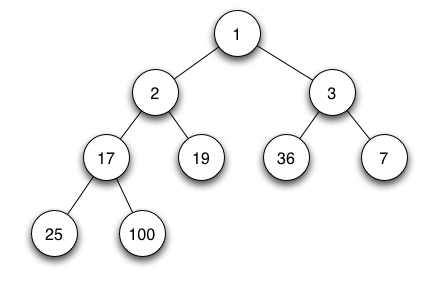
\includegraphics[width=0.6\textwidth]{min-heap.png}}
  \caption{Пример заполненной кучи для минимума}
  \label{pic:min-heap}
\end{figure} 
\AgdaHide{
\begin{code}\>\<%
\\
\>\AgdaKeyword{module} \AgdaModule{HeapDef} \AgdaKeyword{where}\<%
\\
\>\AgdaKeyword{open} \AgdaKeyword{import} \AgdaModule{AgdaDescription}\<%
\\
\>\<\end{code}
}
\section{Тип данных для двоичной кучи}

\subsection{Заполнение дерева}
Куча заполняется элементами слева. Формализуем \cite{HeapFill} заполненность дерева:

\begin{definition}
Двоичное дерево высоты $h$ — \emph{полное} тогда и только тогда,
когда в нем $2^{h+1} - 1$ узлов.

Двоичное дерево высоты $h$ \emph{заполнено слева} тогда и только тогда,
когда выполняется ровно один из пунктов:
  \begin{itemize}
    \item дерево — пустое
    \item дерево — полное (то есть оба его поддерева — либо полные высоты $h-1$, либо пустые)
    \label{def:fill-nd}
    \item его левое поддерево — полное высотой $h-1$ и его правое поддерево — полное высотой $h-2$
    \item его левое поддерево — заполнено слева высотой $h-1$ и его правое поддерево — полное высотой $h-2$
    \item его левое поддерево — полное высотой $h-1$ и его правое поддерево — заполнено слева высотой $h-1$
  \end{itemize}
\end{definition}
Определим вспомогательный тип данных для обозначения заполненности дерева:
\begin{code}\>\<%
\\
\>\AgdaKeyword{data} \AgdaDatatype{TreeState} \AgdaSymbol{:} \AgdaPrimitiveType{Set} \AgdaKeyword{where}\<%
\\
\>[0]\AgdaIndent{2}{}\<[2]%
\>[2]\AgdaInductiveConstructor{full} \AgdaInductiveConstructor{almost} \AgdaSymbol{:} \AgdaDatatype{TreeState}\<%
\\
\>\<\end{code}
Теперь, используя этот тип данных как дополнительный индекс и
индексируя дерево его высотой, задать тип данных для заполненного слева дерева
\begin{code}\>\<%
\\
\>\AgdaKeyword{data} \AgdaDatatype{Tree} \AgdaSymbol{:} \AgdaSymbol{(}\AgdaBound{h} \AgdaSymbol{:} \AgdaDatatype{ℕ}\AgdaSymbol{)} \AgdaSymbol{→} \AgdaDatatype{TreeState} \AgdaSymbol{→} \AgdaPrimitiveType{Set} \AgdaKeyword{where}\<%
\\
\>[0]\AgdaIndent{2}{}\<[2]%
\>[2]\AgdaInductiveConstructor{et} \AgdaSymbol{:} \AgdaDatatype{Tree} \AgdaInductiveConstructor{zero} \AgdaInductiveConstructor{full} \AgdaComment{-- Пустое дерево}\<%
\\
\>[0]\AgdaIndent{2}{}\<[2]%
\>[2]\AgdaInductiveConstructor{nf} \AgdaSymbol{:} \AgdaSymbol{∀} \AgdaSymbol{\{}\AgdaBound{n}\AgdaSymbol{\}} \AgdaSymbol{→} \AgdaSymbol{(}\AgdaBound{a} \AgdaSymbol{:} \AgdaDatatype{Tree} \AgdaBound{n} \AgdaInductiveConstructor{full}\AgdaSymbol{)} \AgdaSymbol{→} \AgdaSymbol{(}\AgdaBound{b} \AgdaSymbol{:} \AgdaDatatype{Tree} \AgdaBound{n} \AgdaInductiveConstructor{full}\AgdaSymbol{)}\<%
\\
\>[2]\AgdaIndent{6}{}\<[6]%
\>[6]\AgdaSymbol{→} \AgdaDatatype{Tree} \AgdaSymbol{(}\AgdaInductiveConstructor{succ} \AgdaBound{n}\AgdaSymbol{)} \AgdaInductiveConstructor{full} \AgdaComment{-- Полное дерево}\<%
\\
\>[0]\AgdaIndent{2}{}\<[2]%
\>[2]\AgdaInductiveConstructor{nd} \AgdaSymbol{:} \AgdaSymbol{∀} \AgdaSymbol{\{}\AgdaBound{n}\AgdaSymbol{\}} \AgdaSymbol{→} \AgdaSymbol{(}\AgdaBound{a} \AgdaSymbol{:} \AgdaDatatype{Tree} \AgdaSymbol{(}\AgdaInductiveConstructor{succ} \AgdaBound{n}\AgdaSymbol{)} \AgdaInductiveConstructor{full}\AgdaSymbol{)} \AgdaSymbol{→} \AgdaSymbol{(}\AgdaBound{b} \AgdaSymbol{:} \AgdaDatatype{Tree} \AgdaBound{n} \AgdaInductiveConstructor{full}\AgdaSymbol{)}\<%
\\
\>[0]\AgdaIndent{6}{}\<[6]%
\>[6]\AgdaSymbol{→} \AgdaDatatype{Tree} \AgdaSymbol{(}\AgdaInductiveConstructor{succ} \AgdaSymbol{(}\AgdaInductiveConstructor{succ} \AgdaBound{n}\AgdaSymbol{))} \AgdaInductiveConstructor{almost} \AgdaComment{-- Полные поддеревья разной высоты}\<%
\\
\>[0]\AgdaIndent{2}{}\<[2]%
\>[2]\AgdaInductiveConstructor{nl} \AgdaSymbol{:} \AgdaSymbol{∀} \AgdaSymbol{\{}\AgdaBound{n}\AgdaSymbol{\}} \AgdaSymbol{→} \AgdaSymbol{(}\AgdaBound{a} \AgdaSymbol{:} \AgdaDatatype{Tree} \AgdaSymbol{(}\AgdaInductiveConstructor{succ} \AgdaBound{n}\AgdaSymbol{)} \AgdaInductiveConstructor{almost}\AgdaSymbol{)} \AgdaSymbol{→} \AgdaSymbol{(}\AgdaBound{b} \AgdaSymbol{:} \AgdaDatatype{Tree} \AgdaBound{n} \AgdaInductiveConstructor{full}\AgdaSymbol{)}\<%
\\
\>[0]\AgdaIndent{6}{}\<[6]%
\>[6]\AgdaSymbol{→} \AgdaDatatype{Tree} \AgdaSymbol{(}\AgdaInductiveConstructor{succ} \AgdaSymbol{(}\AgdaInductiveConstructor{succ} \AgdaBound{n}\AgdaSymbol{))} \AgdaInductiveConstructor{almost} \AgdaComment{-- Правое поддерево — полное}\<%
\\
\>[0]\AgdaIndent{2}{}\<[2]%
\>[2]\AgdaInductiveConstructor{nr} \AgdaSymbol{:} \AgdaSymbol{∀} \AgdaSymbol{\{}\AgdaBound{n}\AgdaSymbol{\}} \AgdaSymbol{→} \AgdaSymbol{(}\AgdaBound{a} \AgdaSymbol{:} \AgdaDatatype{Tree} \AgdaBound{n} \AgdaInductiveConstructor{full}\AgdaSymbol{)} \AgdaSymbol{→} \AgdaSymbol{(}\AgdaBound{b} \AgdaSymbol{:} \AgdaDatatype{Tree} \AgdaBound{n} \AgdaInductiveConstructor{almost}\AgdaSymbol{)}\<%
\\
\>[0]\AgdaIndent{6}{}\<[6]%
\>[6]\AgdaSymbol{→} \AgdaDatatype{Tree} \AgdaSymbol{(}\AgdaInductiveConstructor{succ} \AgdaBound{n}\AgdaSymbol{)} \AgdaInductiveConstructor{almost} \AgdaComment{-- Левое поддерево — полное}\<%
\\
\>\<\end{code}
Для удобства будем называть заполненное слева дерево, индексированное \DC{almost}
\emph{неполным}.

\section{Вставка элементов}
\label{sec:insert}

\subsection{Вставка элементов в полное дерево}
\label{sec:finsert}
\subsection{Вставка элементов в неполное дерево}
\label{sec:ainsert}

\section{Удаление элементов}
\label{sec:delete}
\subsection{Удаление из полного дерева}
\subsection{Удаление из неполного дерева}

% \begin{figure}[h!]
%   \center{\includegraphics[width=0.5\textwidth]{branch_distance.pdf}}
%   \caption{Блок-схема для листинга~\ref{lst:branch_distance}. Малиновым цветом выделена целевая траектория выполнения.}
%   \label{branch_distance}
% \end{figure}

% \section{todo3}

% \subsection{subsection}

% \subsection{}
% \section{}

\section{Выводы по главе \ref{chapter2}}
Разработаны типы данных для представления структуры данных двоичная куча.
